\section{Method}

Different architectures can be adopted to design an agent program implementing the underlying agent function mapping from percept histories to actions. Given the necessity to operate in a partially observable and dynamic environment in a proactive fashion, we based our implementation on the Belief-Desire-Intention (BDI) framework. By explicitly representing the agent's beliefs, desires and intentions, the BDI model allows the agent to reason about its environment, its goals and its own internal state, and to plan and act accordingly.

The pseudo-code of Algorithm~\ref{alg:agent} provides an high-level overview of the main parts of the agent program. After initializing its belief base (denoted as $B$) and its goals (denoted as $D$) based on its initial percepts, the agent enters the main control loop. At each iteration, the agent updates its set of beliefs based on its current observation of the surrounding environment and on the observations made by the agents cooperating with it. The newly updated belief base is then used to revise the agent's desires that are promptly exchanged with the other member of its team. Based on its own internal state and on the desires of the other agents, the agent then select from its set of desires the one to pursue. The chosen intention together with the current knowledge of the environment is then used to formulate a plan (i.e. a sequence of actions) to perform in order to achieve the intention. Finally, the agent executes the first action of the plan, updates its belief base based on the effects of the action. Given the highly dynamic nature of the environment, a cautious approach is adopted, where the agent never commits to execute a plan in its entirety, but instead re-evaluates its desires and intentions after each action.

\begin{algorithm}
    \caption{Agent control loop}
    \label{alg:agent}
    \begin{algorithmic}
        \item \textbf{Input:} $B_0$ (initial belief base)
        \State $B \gets$ $B_0$
        \State $D \gets$ options($B$)
        \While{true}
        \State perceive $o$
        \State $o \gets$ exchangeObservations($o$)
        \State $B \gets$ update($B$, $o$)
        \State $D \gets$ revise($D$, $B$)
        \State $D \gets$ exchangeDesires($D$)
        \State $I \gets$ select($B$, $D$)
        \State $P \gets$ plan($B$, $I$)
        \State $\alpha \gets$ head($P$)
        \State $r \gets$ execute($\alpha$)
        \State $B \gets$ update($B$, $r$)
        \EndWhile
    \end{algorithmic}
\end{algorithm}

Before delving into the details of the implementation, some clarifications need to be made. While for the sake of simplicity we have presented the agent control loop as a sequential process, in practice most of the operations are performed concurrently. Indeed, this is a paramount requirement in a highly dynamic environment such as the one of the Deliveroo game, where changes in the environment can happen even while the agent is reasoning, planning and acting. Thus, all perceptions, communications and updates are performed asynchronously and in an event-driven fashion such that updates to the belief base and the desires are performed as soon as new information is available.


\subsection{Team Communication}

As stated in the introduction, not all agents in the environment are adversarial. In fact, agents may form teams and cooperate with each other to better achieve their goals. To allow the formation of teams and the exchange of information among the agents (necessary for an effective and productive cooperation), a communication protocol has been implemented.

The protocol is built upon two communication primitives made available to the agents by the engine: \texttt{shout} and \texttt{say} (a third primitive, \texttt{ask}, is also available, but it has not been used in our implementation). The \texttt{shout} primitive allows the agent to broadcast a message to all the agents in the environment, while the \texttt{say} primitive allows the agent to send a message to a specific agent. Even though the provided communication channels are unreliable (i.e. there is no guarantee about when or if the message will be received), no reliability layer has been implemented on top of them, as the agents are designed to be robust to temporary communication failures. In fact, temporary inconsistencies in the belief bases of the team members should not impact the overall performance of the team in the long run.

Since agents do not know in advance which other agents are in the environment and which of them are adversarial or cooperative, the first step of the communication protocol is to establish the identity of the agents and to form teams. To this end, each agent broadcasts a \texttt{hello} message to all the agents in the environment. Since agents may appear at any time during the game, the \texttt{hello} message is periodically broadcasted. To allow the receiving agent to verify that the sender of the message is indeed a legitimate agent, the \texttt{hello} message contains the id of the sender encrypted using the AES-256 algorithm with a secret key known only to the agents of the same team. Upon receiving a \texttt{hello} message, the receiving agent can verify whether the decrypted id matches the id of the sender and, if so, it can add the sender to its set of cooperating agents. In this way, even if a malicious agent intercepts the \texttt{hello} message and tries to replay it, the receiving agent will notice that the id of the sender does not match the decrypted id and will discard the message.

The other part of the communication protocol regards the exchange of information among the agents in the same team. To avoid adversarial agents from exploiting the information exchanged among the team members, the following messages are not broadcasted to all the agents in the environment, but are instead sent only to the agents in the same team. Moreover, to avoid malicious agents from injecting false information in the belief bases of the team members, messages sent by non-cooperating agents are ignored. To this messages no encryption is applied since the \texttt{say} primitive should already guarantee that the message is received only by the intended recipient.

The exchange of information regards three main aspects: the observations of the environment, the desires of the agents, and the position of the agents.

The observation of the environment is the main source of information for the agents to update their belief bases (see Section~\ref{sec:belief-base} for more details). Each time an agent receives a new observation of the environment, it relays the observation to the other agents in the team. By doing so, the belief bases of the agents in the same team are kept in sync and their knowledge of the environment is both more accurate and more complete. One could argue that it would be better to only relay updates to the belief base, rather than each observation (which are much more frequent). However, we noticed that this leads to a higher risk of inconsistencies since temporary inaccuracies in the belief base of one agent will be propagated to all the other agents in the team.

As for the observations, each time an agent updates its desires, it relays the new desires to the other agents in the team. In this way, the agents in the team can coordinate their actions and not interfere with each other (e.g. by not picking up the same parcels) to better achieve their goals. Finally, each time the position of an agent changes, it relays its new position to the other agents in the team.


\subsection{Belief base}
\label{sec:belief-base}

In the BDI model, the belief base represents the information that the agent has about the world. In the context of the Deliveroo game, the informational state of the agent includes both the ground truth facts about the environment and the agent's own beliefs about the current state of the world. The former includes the topology of the map, the location of the pickup and delivery locations, and other parameters controlling the game dynamics. The latter includes the agent's beliefs about the state of the parcels and the other agents, as well as the agent's own state (e.g. its current location and its membership to a team). While the ground truth facts are fixed and given as input to the agent when the game starts, the agent's beliefs require to be constantly updated based on the received observations so as to maintain the most accurate representation of the world on which to reason and plan.

Hereafter, we describe the main assumptions and design choices made to keep track of the changes in the environment and to update the belief base accordingly.

\paragraph*{Parcels}
One of the main components of the belief base is the set of parcels that the agent can pickup (that is, the parcels that are not yet picked up by any agent). Each parcel is represented as a tuple $(p, l, t, v)$, where $p$ is a unique identifier, $l$ is the location of the parcel, $t$ is the time at which the parcel was first observed, and $v$ is the value of the parcel at time $t$ (by knowing the time at which the parcel was first observed, the agent can estimate the current value of the parcel based on its decay rate).

Each time the agent receives a new observation (from its sensors or from the sensors of the other team members), it updates the set of parcels in its belief base accordingly. In particular, if the agent observes a free parcel that it was not aware of, it adds the parcel to its belief base. If the agent observes a parcel that it was already aware of but in a different location or now picked up by another agent, it updates its location or removes it from its belief base accordingly. Given that the agent can only perceive its surroundings within a certain radius, the state of the parcels that are not within the team's perception range can not be determined with certainty. In such case, we decided to mark as no longer free only those parcels whose last observed location is inside the perception range but that are not currently observed by any agent in the team.

\paragraph*{Agents}
Tracking the state of the other agents is also a crucial part as their positions and intentions can greatly affect the agent's own plans. Here a distinction must be made between the agents in the same team and the adversarial agents. Tracking the state of the cooperating agents is straightforward, as their position and desires are directly communicated by the agents themselves. The only additional information that the agent needs to keep track of is the last time at which the agent has sent a message to the team. This is necessary to detect when an agent has been inactive for too long and remove it from the team.

On the other hand, keeping the belief base up-to-date with the state of the adversarial agents is more challenging as we can only rely on the observations made by the agent itself and its team. Each of the adversarial agents is represented as a tuple $(a, l, t, r)$, where $a$ is a unique identifier, $l$ is the last observed location of the agent, $t$ is the time at which the agent was last observed, and $r$ is a boolean flag indicating whether the agent is considered a random agent. Note that by random agent we do not necessarily mean an agent that moves randomly (i.e. without any specific goal), but an agent whose behavior does not seem to be rational (i.e. whose actions do not seem to be aimed at maximizing its reward).

Each time the agent receives a new observation, it updates the set of adversarial agents in its belief base accordingly. In particular, if the agent observes a new agent, it adds the agent to its belief base, otherwise it updates the last observed location and the last observed time of the agent. Given that the agent can only perceive its surroundings within a certain radius, the state of the adversarial agents that are not within the team's perception range can not be determined with certainty. In such case, since agents are much more dynamic than parcels, we decided to mark as undefined the position of all agents that have not been observed for a certain amount of time. This is done to avoid the agent to make decisions based on outdated information.

To assess whether an agent is randomly moving, a simple heuristic has been defined. If from the first time the agent was observed to the last time it was observed its score is below a certain threshold, the agent is considered a random agent. The threshold is defined as the expected reward a greedy agent would have obtained in the same time span. This is computed in the following way:

\begin{equation*}
    \mathbb{E}_{\text{greedy}}[r] = \frac{\mathbb{E}[dist]}{\mu_{\texttt{dist}}} \cdot \frac{\mu_{\texttt{reward}}}{n_{\texttt{smart}}}
\end{equation*}

where $\mathbb{E}[dist]$ is the expected distance covered by the agent in the time span, $\mu_{\texttt{dist}}$ is the average distance between parcels in the map, $\mu_{\texttt{reward}}$ is the average reward of the parcels, and $n_{\texttt{smart}}$ is the number of agents in the environment that are not random agents.

Finally, note that here we do not make any assumption about the possible intentions of other agents. Indeed, modelling the behaviour of other agents is a complex and challenging task that may require learning-based approaches. Therefore, we preferred not to implement any partial model of the other agents' intentions, given that wrong assumptions about the actions of the other agents can lead to sub-optimal decisions.


\subsection{Search Tree}
\label{sec:search}

In the BDI model, the desires represent the goals that the agent wants to achieve. In the context of the Deliveroo game, at each time instant the goals of the agent are to move to a location where there are parcels or to deliver the currently held parcels (if any). Therefore, each time there is a change in the set of available parcels, the agent needs to update its desires accordingly.

Since the long-term objective of the agent is to maximize its reward, not all desires are equally important and worth pursuing. Therefore, it is necessary to assign them a score that should reflect their goodness for the agent's long-term goal. Hence, we deemed not sufficient to assign them a score based on their immediate reward, as this would lead the agent to be short-sighted and not to take into account the future consequences of its actions. To avoid this, we decided to implement a forward-looking scoring function based on Monte Carlo Tree Search. By using the MCTS algorithm, the score of each desire depends not only on the immediate reward, but also on the expected future reward that the agent can obtain after pursuing the desire.

Hereby we describe the main design choices and modifications made to the MCTS algorithm to make it more suitable for a highly dynamic and real-time environment such as the Deliveroo game.

Instead of searching over all possible move actions (up, down, left, right) that the agent can perform, to reduce the search space and to make the search more efficient, we decided to search over the possible desires that the agent can pursue at a given time instant. Thus, moving from one node of the search tree to another corresponds to pursuing a desire and each node corresponds to the state of the game if the agent were to execute all the desires along the path from the root node to the current node. Thus, we have that the root node corresponds to the current state of the game, its children correspond to the possible desires that the agent can pursue at the current time instant (among which the agent will choose the best one to pursue), the children of each child correspond to the remaining possible desires that the agent can pursue after pursuing the desire corresponding to the parent node, and so on.

With respect to standard applications of MCTS, we decided not to model the state of the game that is not under our control, except for the decaying of the parcels. In fact, while MCTS is often used to model processes where the only uncertainty is given by the opponent's actions, in the Deliveroo game the uncertainty is much higher and computing the full state would require modelling the behaviour of other agents and the dynamics of the environment.

Since we no longer model the randomness of the environment, the utility is no longer an expectation over the possible outcomes of the game, computed as the average of the rewards obtained by simulating the game from the node state. Instead, the utility of a node is the exact reward that the agent can obtain from the given state of the game. Since we are interested in the best desire to perform, the utility of a node is equal to the maximum utility of its children plus the immediate reward the agent can obtain by pursuing the desire corresponding to the node. In particular, if the desire is a pick-up then its immediate reward is 0 (since the agent does not obtain any reward by picking up a parcel), while if the desire is a delivery then its immediate reward is the value of the delivered parcels (at the time of the delivery).

Since the search must satisfy real-time constraints, some optimizations have been made to make it more efficient. First of all, in the play-out phase (i.e. the phase in which the game is simulated from the current state to the end), instead of throwing away the simulated subtree at the end of the play-out, we decided to keep it. While this increases the memory usage, it allows the agent to reuse the subtree in the next iterations of the search without having to recompute it from scratch. Furthermore, since before selecting the best desire to pursue the number of played iterations may be limited, we decided to expand the children of a node based on their greedy score (i.e. the reward obtained by pursuing that desire followed by a putdown) as to focus the first iterations of the search on the most promising desires.

Finally, in traditional applications of MCTS, the search is restarted from scratch after each move. Doing the same in our case would be too inefficient and would not allow the agent to reuse the information gathered in the previous iterations of the search. Therefore, we decided to adopt a dynamic search strategy, in which the tree is modified in place as the game progresses. In particular, each time the agent moves the state of the root node is updated with the new position, while, when the agent completes a desire, its corresponding child is promoted to the root node and the other children are discarded. Furthermore, as new parcels appear or disappear, the nodes corresponding to the pick-up desires are added or removed from the tree.

\subsection{Selection}
\label{sec:selection}

The selection phase is the process of choosing which desire to pursue next. As stated above, the possible desires that the agent can pursue at the current time instant correspond to the children of the root node of search tree. Thus, the most intuitive way to select the desire to pursue would be to choose the desire with the highest score. However, given the presence of other agents in the environment, the choice of the next intention must necessarily take into account the state of the other agents and the desires of the other team mates.

To take into account the state of the non-cooperating agents, the score of each desire is adjusted based on how likely the agent can achieve it without being interfered by the other agents. To this end, the score of each pick-up desire is decreased if there are other agents in the vicinity that are more likely to pick up the same parcels first. This is done by decreasing the score of the desire by a factor inversely proportional to the distance of the closent adversarial agent to the pick-up location. More formally, the score of each desire is adjusted as follows:

\begin{align*}
    \texttt{factor} & = 1 - \frac{1}{1 + \min_{a \in A} \texttt{dist}(a, l)} \\
    \texttt{score}  & = \texttt{score} \cdot \texttt{factor}^2
\end{align*}

where $A$ is the set of non-random adversarial agents, $l$ is the location of the parcel, and $\texttt{dist}(a, l)$ is the distance between the agent $a$ and the location $l$.

To make the cooperation among the team members more effective, we need to ensure that no team members are pursuing the same desire at the same time. Even better, we should try to distribute the work among them such as to maximize the overall reward. To find the best one-to-one assignment of the desires to each team member Hungarian Matching \parencite{hungarian} has been used. Since the intention to pursue is recomputed after each action, to avoid a frequent reassignment of desires among team members, the score of a desire (for the next time instant) is adjusted based on the current assignment of desires to the team members. In particular, the score of each desire is decreased if it has been previously assigned to another team member, while it is increased if it has been previously assigned to the agent itself.

A particular case that needs to be handled is when the agent is carrying some parcels but it cannot reach any delivery location. In such case, the agent sends a \texttt{ignore-me} message to the other agents in the team to inform them that it should not be taken into account when assigning the desires to the team members. Meanwhile, the agent will start moving towards its nearest team mate to deliver the parcels to them. As soon as the agent delivers the parcels, it sends a \texttt{resume-me} message to the other agents in the team to inform them that it should be taken into account again when assigning the desires to the team members.

Finally, it may happen that the reward the agent can obtain by pursuing the chosen intention is not worth the effort. In such cases, it would be better to move to another location of the map hoping to find better opportunities. To this end, when the score of the chosen intention is equal to 0, the agent starts moving to the most promising position of the map. To find the most promising position a simple heuristic has been defined. Intuitively, a position on the map is more promising if it is close to a spawning point but far from other agents. More formally, the score of each position is computed as follows:

\begin{equation*}
    \texttt{score} = (\sum \limits_{p \in P} e^{-\frac{1}{2}(\frac{\texttt{dist}(p, l)}{\sigma})^2}) \cdot \prod \limits_{a \in A} (1 - e^{-\frac{1}{2}(\frac{\texttt{dist}(a, l)}{\sigma})^2})
\end{equation*}

where $P$ is the set of spawning points, $A$ is the set of all agents, $l$ is the location of the position, $\texttt{dist}(p, l)$ is the Manhattan distance between the spawning point $p$ and the location $l$, and $\sigma$ is a scaling factor that determines the radius of the influence. As can be seen, the score of each position is the product of two terms. The first term is the sum of the positive Gaussian functions centered at the spawning points, while the second term is the product of the negative Gaussian functions centered at the other agents.


\subsection{Planning}

Once the intention to pursue has been selected, the agent needs to formulate a plan to achieve the intention. In the case of the Deliveroo game, the plan consists of a sequence of move actions (up, down, left, right) to perform to reach the desired location. In other words, the planning problem can be seen as a shortest path problem on a two-dimensional grid.

Given that the computation of the shortest path is often required (after each action and during the whole search phase), recomputing the shortest path from scratch each time would be both inefficient and unnecessary. Therefore, considering also the fact that the map layout does not change except for the position of the agents, we decided to precompute the shortest path from each tile to each other tile of the map and to store the results in a look-up table. To this end, we decided to adopt the Seidel's algorithm~\parencite{seidel} to compute the shortest path between each pair of tiles. By treating the map as an undirected and unweighted graph (where each walkable tile is a node and each edge connects two adjacent tiles), the algorithm computes the shortest distance (that can be easily used to compute the shortest path) between each pair of nodes in $O(V^{\omega} log(V))$ time, where $V$ is the number of nodes and $\omega$ is the exponent of matrix multiplication. Given that the number of nodes in the map is relatively small, the precomputation of the lookup table can be performed in a reasonable amount of time that will be repaid by the speedup in the planning phase.

As stated above, the precomputed paths do not take into account the current state of the environment, that is the occupied positions. Thus, when the agent perform the first move of the plan, it may find the destination tile to be occupied by another agent. In such case, the agent needs to recompute the shortest path to the destination tile, taking into account the current state of the environment. To this end, we decided to leverage a PDDL planner to give us a viable path. In our case, the PDDL domain is relatively simple as the only possible actions are up, down, left, right while the PDDL problem is created taking into account the agents' positions every time there is the need to recompute the path. As the planning computation needs to be performed in real-time, rather that using the provided online planner (that would introduce further latency), we decided to use the Planutils tool \parencite{planutils} to locally run the FF PDDL planner.

To further speed up the planning phase, we also implemented a  solution based on the A* search algorithm \parencite{a*}. By further exploiting the precomputed distances as the heuristic function (an admissible and consistent heuristic), the A* search is guaranteed to find the shortest path in the most efficient way.

\begin{figure}
    \centering
    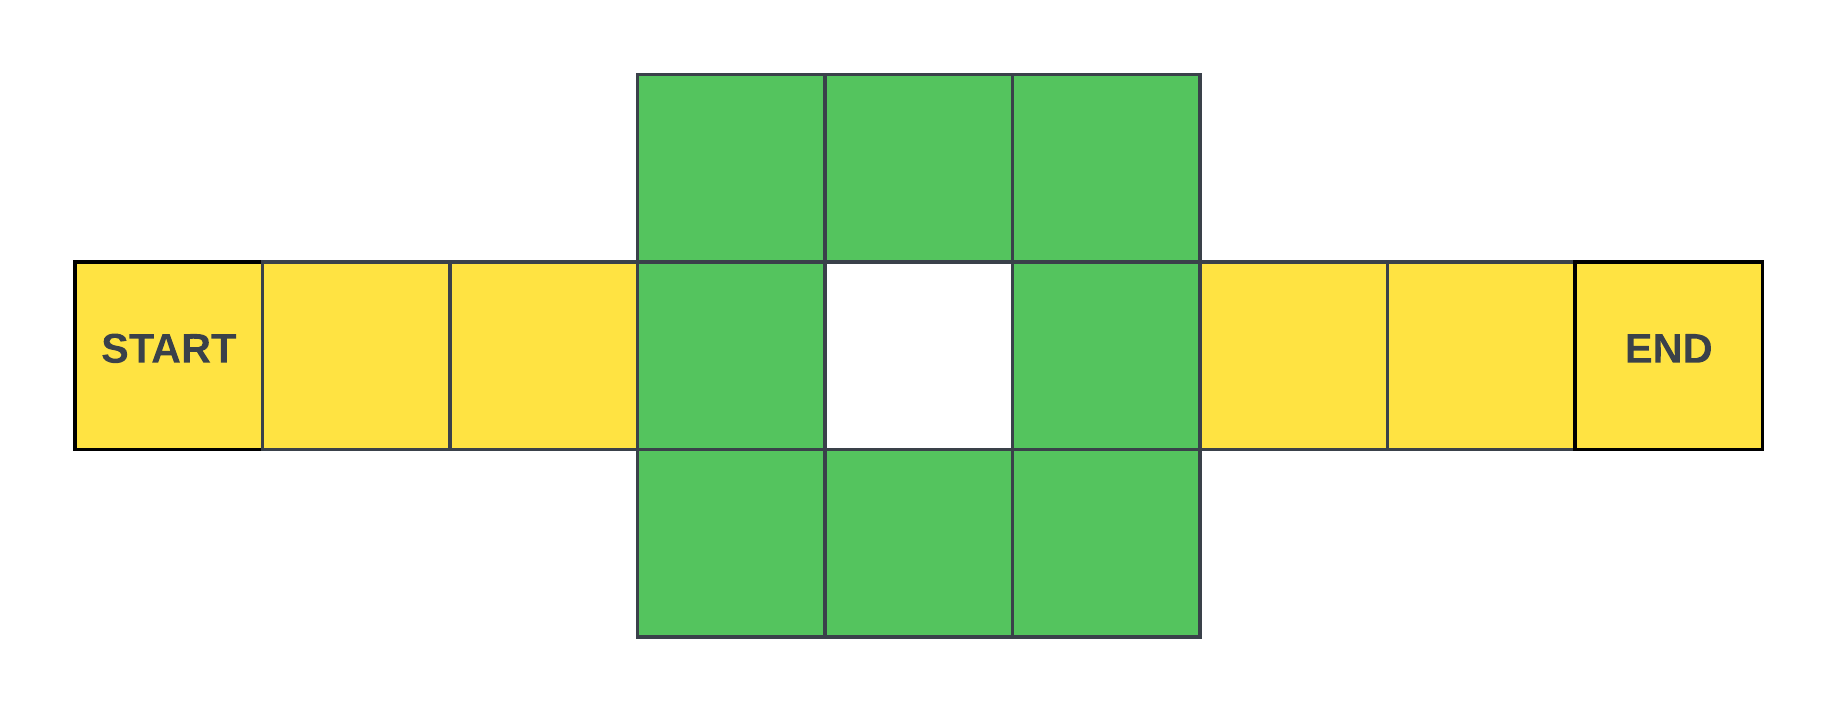
\includegraphics[width=0.49\textwidth]{figures/path-bottleneck.png}
    \caption{An example of path bottleneck. The tiles in yellow belong to the path bottleneck from the start position to the end tile.}
    \label{fig:path-bottleneck}
\end{figure}

The recomputed paths are then stored in a cache to be reused in the future. However, given the highly dynamic nature of the environment, an invalidation mechanism has been implemented to remove from the cache the paths no longer valid. To this end, the concept of path bottleneck is introduced. When moving from the current position to the destination tile, the set of all tiles that the agent must necessarily traverse to reach the destination in the shortest time is called the path bottleneck (see Figure~\ref{fig:path-bottleneck}). In other words, the path bottleneck is equal to the intersection of all the shortest paths from the current position to the destination. Given such definition, it is easy to see that the path recomputation is necessary only when the path bottleneck is no longer free. Thus, as soon as the path bottleneck becomes free again, the recomputed path can be discarded and the Seidel's cache can be used again.